\documentclass[conference]{IEEEtran}
\usepackage{times}
\usepackage[numbers,sort&compress]{natbib}
\usepackage{graphicx}
\usepackage{booktabs}
\usepackage{amsmath,amssymb}
\usepackage{microtype}
\usepackage{xcolor}
\usepackage[colorlinks=true,linkcolor=black,citecolor=black,urlcolor=black]{hyperref}
\newcommand{\tasksall}{105}
\newcommand{\clipsall}{21}
\newcommand{\causeGoal}{0.00}
\newcommand{\causeTrackerClip}{0.84}
\newcommand{\causeTrackerAway}{0.05}
\newcommand{\causeRefClip}{0.92}
\newcommand{\causeRefAway}{0.25}
\newcommand{\causeHybridClip}{0.98}
\newcommand{\causeHybridAway}{0.92}
\newcommand{\causeNoTeacher}{With the tracking reward alone, the form of the reference worlds of~\cite{hil,wang2026generalizing}, reference worlds by themselves teach the motion in two of three seeds (0.84 and 0.93 from the clip start; the third learns nothing), and an even split with goal worlds learns nothing in any seed: the failure that~\cite{wang2026generalizing} report for mixing without a schedule. With the teacher the even split reaches 0.98 and 0.92 in every seed (Sec.~\ref{sec:tracker}).}
\newcommand{\scheduleSentence}{It holds 0.8 from displaced starts from 22 million samples in each of the three seeds. The best fixed share needs 37 million, the tracking-progress schedule 43, and two stages 53: 1.7, 2.0, and 2.4 times as many. It reaches the clip-start level as early as any setting, and ends at 0.98 from the clip start and 0.95 from displaced starts. Its share starts at 0.9, because nothing but the motion can be taught yet, falls to 0.2 as the evaluation shows the motion arriving, and then follows what still fails. Without the gates the rule starts at one half and needs 27 million samples.}
\newcommand{\trialSamples}{12 to 27}
\newcommand{\trialCost}{twice}
\newcommand{\displacedHalf}{0.92}
\newcommand{\displacedThreeQuarters}{0.76}
\newcommand{\displacedOne}{0.56}
\newcommand{\displacedTrackerQuarter}{0.23}
\newcommand{\displacedTrackerOne}{0.01}
\newcommand{\lossStarts}{0.69}
\newcommand{\fullTrackerSamples}{590}
\newcommand{\fullTrackerClip}{0.52}
\newcommand{\fullTrackerAway}{0.17}
\newcommand{\fullTrackerSolved}{62}
\newcommand{\fullSentence}{After 590 million samples it succeeds in 0.89 of episodes from the clip start and 0.86 from displaced starts, averaged over the tasks and the two seeds (ranges 0.88 to 0.90 and 0.86 in each), and solves 101 to 103 and 102 to 104 of the \tasksall{} tasks at 0.5 or better. The tracker is at 0.52 and 0.17, and at 62 tasks and one. The policy passes the final clip-start success of its teacher after 221 to 246 million samples of its own, and the share of reference worlds falls from 0.84 to about 0.35 on the way. \fullBaseline{}}
\newcommand{\fullTasksSentence}{The policy solves 39 to 41 tasks from the clip start that its teacher does not, and none the other way in any seed. Among them, in the first seed, are all heights of four clips on which the tracker never completes the climb (0.00 to 0.02 for the tracker, 0.87 to 0.99 for the policy) and most of the tallest boxes (0.33 against 0.86 at the largest scale). Every seed fails the 1.14\,m box.}
\newcommand{\timeSentence}{With the GPU to itself, the tracker of the development clip trains its 74 million samples in 4.1 minutes, and the policy then holds 0.8 from displaced starts 80 seconds into its own training, at 22 million samples; its full 59 million samples take 3.5 minutes. Simulation and learner together run at about 290 thousand samples per second with 4{,}096 training worlds. On all clips, the tracker and the policy each take about 40 minutes for their 590 million samples at the rate they ran while they had the GPU to themselves; the reported runs shared it with other runs for part of their time.}
\newcommand{\abstractSchedules}{on one clip at five box heights the policy reaches 0.8 success from displaced starts after 22 million samples in each of three seeds, 1.7 times fewer than the best fixed share found by a sweep and 2.0 and 2.4 times fewer than two published hand schedules.}
\newcommand{\abstractAll}{One policy trained this way on 105 tasks succeeds in 0.89 of episodes from the starts of the clips and 0.86 from displaced starts (mean of two seeds), where the tracker that teaches it reaches 0.52 and 0.17, and it solves 39 to 41 tasks that its teacher does not.}
\newcommand{\fullBaseline}{With an even share and tasks drawn evenly, the usual setting, the same budget ends at 0.72 and 0.65 with 81 and 69 tasks solved in its one seed, and the policy needs 344 million samples to reach a mean of 0.5 from the clip start, against 221 to 246 million with the rule.}
\newcommand{\heldoutSentence}{With the box heights at scales 0.9 and 1.1 held out of every clip, the policy succeeds on them in 0.90 of episodes from the clip start and 0.81 from displaced starts, as on the heights it trained on (0.87 and 0.80): it interpolates over box height. With five of the \clipsall{} clips held out, it succeeds in 0.48 and 0.46 on climbs it has no reference for, against 0.83 and 0.80 on the clips it trained on. That mean hides a split: two of the five clips are solved at every height, one at none, and two in part.}
\newcommand{\noTeacherSentence}{With the tracking reward alone, the climb is learned in four of the seven runs that begin with reference worlds only (reference worlds alone, two stages, tracking progress) and in none of the eight that have goal worlds from the first iteration. The credit rule is among the latter: it starts with a tenth of its worlds on goals, and without the teacher it learns nothing in three seeds. With the teacher, all 27 runs with a share of at least 0.25 learn. The teacher is therefore what the rule relies on. It turns a first stage that succeeds about half of the time into one that always does, and it lets goal worlds be present from the start.}
\newcommand{\seedsAll}{two}


\newcommand{\ours}{\textsc{Credit}}

\begin{document}

\title{Credit the Cause: Evaluation-Driven Allocation of\\Simulated Worlds for Humanoid Box Climbing}

\author{\IEEEauthorblockN{Anonymous Authors}}

% The first figure sits under the title, across both columns.
\makeatletter
\let\titleonly\@maketitle
\renewcommand{\@maketitle}{\titleonly
  \begin{center}
  \def\@captype{figure}\setcounter{figure}{0}
  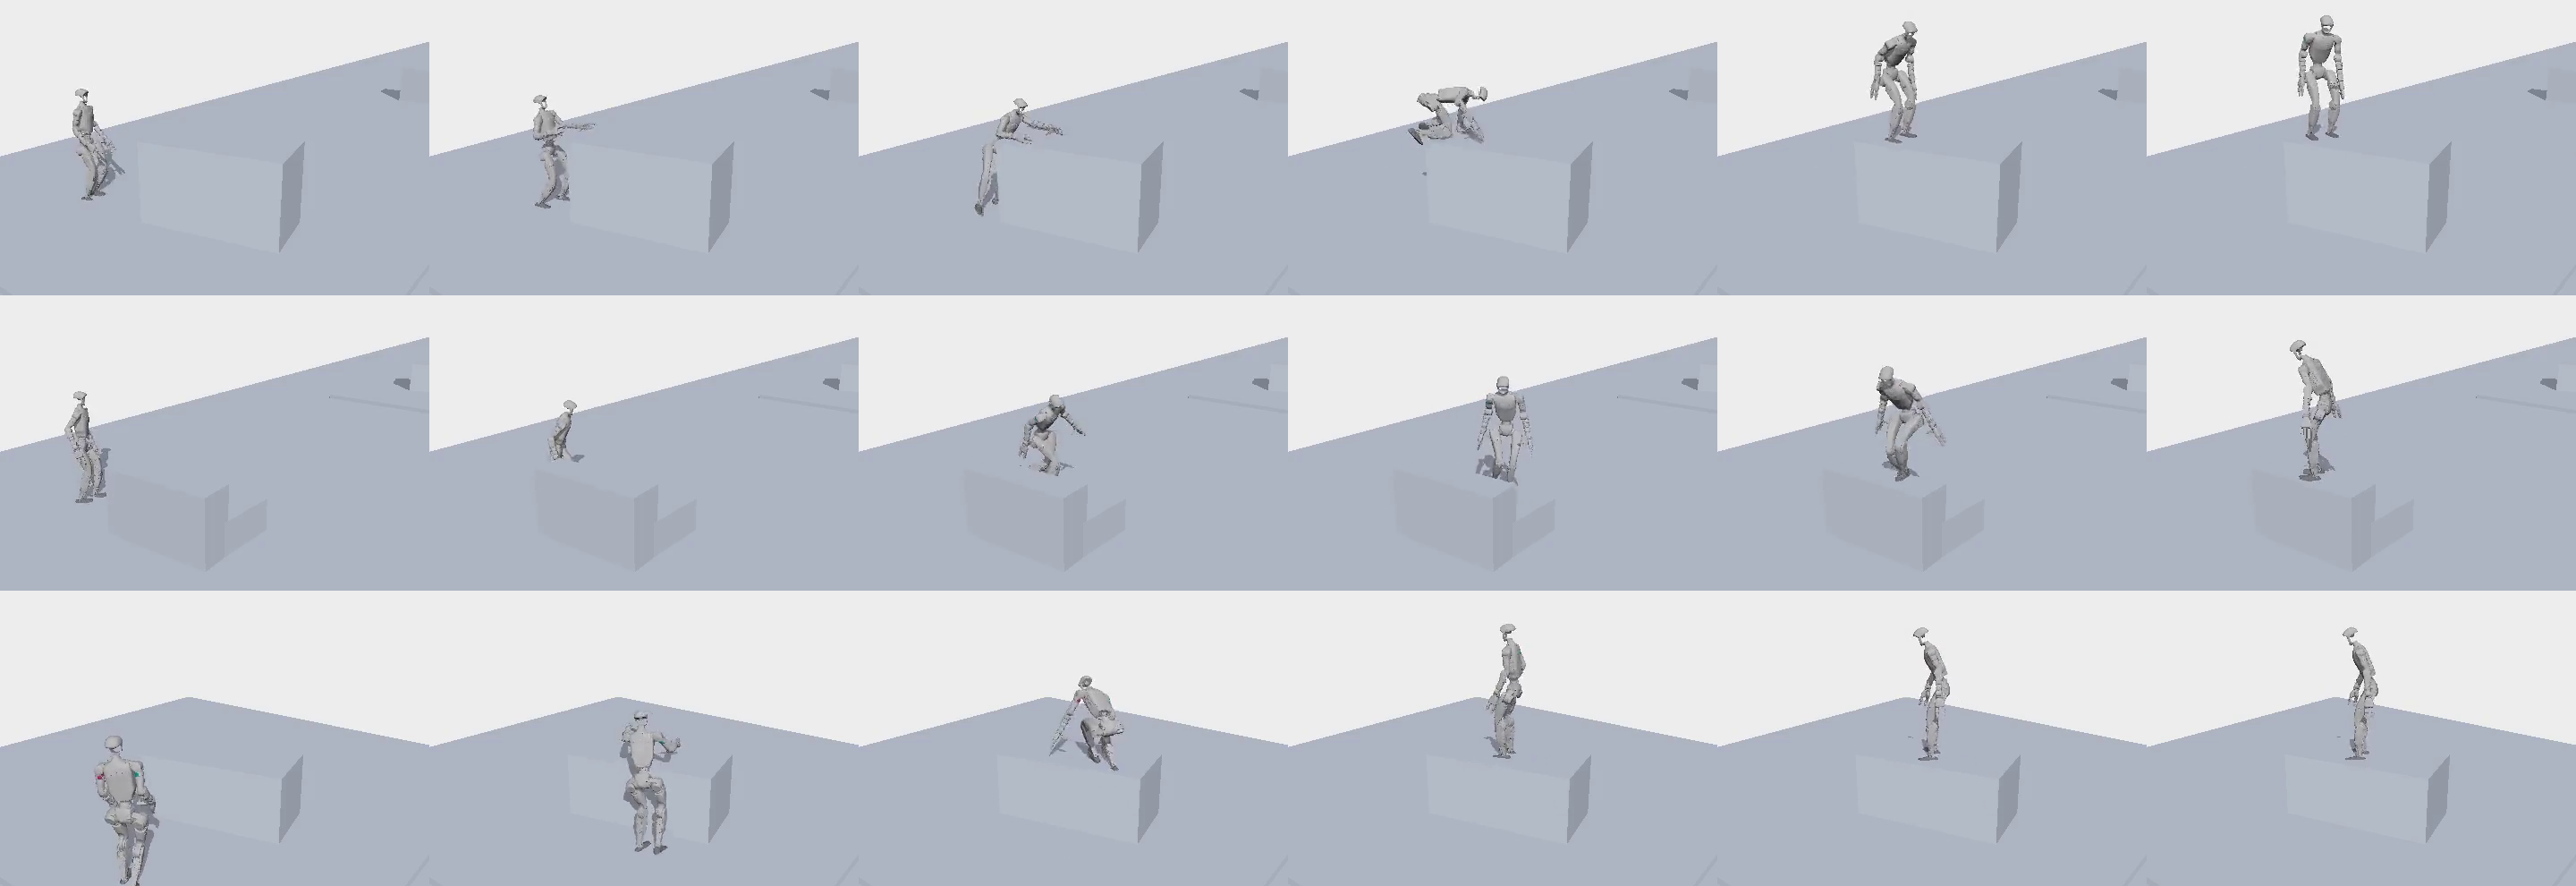
\includegraphics[width=\textwidth]{figs/teaser.png}
  \caption{One policy climbs three of its \tasksall{} tasks from starts that the clips do not contain: a 0.95\,m box, two boxes of 0.35 and 0.70\,m, and a 0.72\,m box (six frames over each episode, left to right). The policy observes the robot, a height scan, and the goal pose. It never observes a clip, and its only task reward is one Boolean at the end of the episode.}
  \label{fig:teaser}
  \end{center}}
\makeatother

\maketitle

\begin{abstract}
A tracker makes a humanoid climb a box by following a clip, but it needs the clip to act and fails when the robot starts elsewhere. A goal-driven policy adapts to its start, but a reward that only says whether the robot stands on the box teaches nothing. Hybrid methods train both objectives in parallel worlds of one simulation and set the split between them by hand. We ask instead what the worlds of each kind cause, measure it in evaluation worlds inside the training simulation, and allocate worlds by it. On a Unitree G1 climbing boxes of 0.38 to 1.14\,m from public clips, worlds with the Boolean alone learn nothing; worlds that imitate a tracker give a policy that never sees a clip the motion, but not its use away from the clip; both together give both. The share of each kind is a strong, one-sided lever with a moving optimum. A rule that reads only the evaluation worlds sets it with no schedule and no cost: \abstractSchedules{} \abstractAll{} All results are in simulation.

\end{abstract}

\IEEEpeerreviewmaketitle

\section{Introduction}

A humanoid that climbs onto a waist-high box uses its hands, knees, and shins, in an order that is hard to find by trial and error and easy to see in a person doing it. Two families of methods turn that observation into a controller, and each gives up something. \emph{Trackers} follow a retargeted clip frame by frame~\cite{deepmimic,beyondmimic,zest,omniretarget}. They reproduce the motion, but they need the clip at deployment and fail when the robot does not start where the clip does. \emph{Goal-driven} policies are told only where to end up, so they adapt to where they start, but a reward that says only ``you stand on the box'' gives no signal until the robot stands on the box, and the shaped rewards that replace it are engineered per behaviour.

Hybrid methods train both objectives at once, in parallel worlds of one simulation that share a policy~\cite{hil,wang2026generalizing}. Their results agree on two points. The mixture matters enormously: with a sparse goal reward, removing the reference worlds takes success on box jumps and climbs from 1.00 to 0.00~\cite{wang2026generalizing}, and adding goal worlds before the policy can follow the references does the same. And the mixture is set by hand: a fixed number of samples of tracking followed by an even split~\cite{hil}, or a schedule driven by how well the policy tracks~\cite{wang2026generalizing}. Neither measures what the reference worlds do for the goal task, which is the reason they are there.

This paper asks what the worlds of each kind \emph{cause}, measures it inside the training simulation, and allocates worlds by it. We call the principle \emph{credit the cause}: a kind of world receives worlds for the failures of the evaluation that it has been measured to remove, in the tasks where it is able to remove them. The system has three kinds of worlds (Fig.~\ref{fig:system}). \emph{Reference worlds} start on a frame of a clip and imitate a tracker. \emph{Goal worlds} start on a frame of a clip or away from it and receive one Boolean at the end of the episode: whether the robot stands at the goal. \emph{Evaluation worlds} run the policy without exploration noise on every task from a fixed ladder of starts and give nothing to the learner. Their Booleans are the only signal the allocation reads.

We study the Unitree G1 climbing onto and over boxes of 0.38 to 1.14\,m, with the clips and boxes of a public dataset~\cite{omniretarget}. The policy we train never sees a clip: it observes the robot, a height scan of the terrain, and the pose of the goal. Our contributions are:
\begin{itemize}
\item A measurement of what each kind of world causes. Goal worlds alone learn nothing in the budget we tested, not even to stand. A tracker reaches the goal from the first frame of its clip and almost never from starts half a metre away. Reference worlds alone give a clip-free policy the motion but not the adaptation. Goal worlds added to them give both (Sec.~\ref{sec:cause}).
\item Evidence that the share of worlds of each kind is a strong and one-sided lever: with a tenth of the worlds on references nothing is learned, with all of them the policy stays tied to the clip, and the best share moves during training (Sec.~\ref{sec:share}).
\item An allocation rule that reads only the evaluation worlds and costs nothing. It needs no schedule, and reaches our success levels in 1.7 times fewer samples than the best fixed share found by a sweep and 2.0 to 2.4 times fewer than two published hand schedules (Sec.~\ref{sec:schedules}). Two learners that try neighbouring shares in parallel measure the same direction directly, at twice the samples.
\item One policy for \tasksall{} box-climbing tasks from public data. It solves 103 of them from the starts of the clips and 104 from displaced starts, against 62 and one for the tracker that teaches it, and 41 tasks that the tracker does not solve at all (Sec.~\ref{sec:all}).
\end{itemize}
All results are in simulation; we state what we did not test in Sec.~\ref{sec:limits}.

\section{Related Work}

\textbf{Tracking and its data.} DeepMimic~\cite{deepmimic} established reward-driven tracking of a reference with starts on its frames. Recent trackers scale it to hardware and to contact-rich skills~\cite{beyondmimic,zest}. OmniRetarget~\cite{omniretarget} generates clips of a G1 on terrain that preserve the contacts of the human, and releases those we use. A tracker needs its reference to act. Distillation removes it at deployment by training a student on the tracker's actions under a sparser interface~\cite{maskedmimic,hover}, the DAgger scheme~\cite{dagger}; the student is then trained only on what the tracker visits.

\textbf{Imitation with goals.} Adversarial priors add a style reward to a task reward~\cite{amp,amphardware}; on a parkour course, starting them from scratch completes 0.11 of the courses against 0.85 after a tracking stage~\cite{hil}. HIL~\cite{hil} runs tracking worlds and goal worlds in parallel with one observation space, after four billion samples of tracking alone. Wang et al.~\cite{wang2026generalizing} train a G1 on box jumps and climbs with imitation worlds and goal worlds whose reward is sparse, one policy per behaviour; a scalar that follows tracking success lowers the share of imitation worlds from 1.0 to 0.5 and removes an assistive force. ConsMimic~\cite{consmimic} adapts the weight of a style reward to keep the task return near its best, and notes that it cannot tell which parts of the demonstrations help. We keep the parallel worlds of these methods, supervise the reference worlds with a tracker instead of a tracking reward alone, and set the split from what evaluation worlds measure.

\textbf{Curricula and samplers.} Success Guided Sampling~\cite{sgs} samples a fixed set of task configurations by their own success rate, with a Boolean terminal reward and resets that reach near the goal~\cite{omnireset}; its ablations show little sensitivity to the parameters of the sampling rule and no learning without the resets near the goal. Learning-progress curricula score a task by the change of its own return~\cite{lpacrl,graves2017automated}. Starts on demonstration states turn a sparse reward into a curriculum~\cite{florensa2017reverse,demostart,scout,goexplore}. These methods choose among tasks or starts of one objective by statistics of the training episodes. We allocate between kinds of supervision, and read held-out evaluation episodes instead. Population-based training~\cite{pbt} selects among learners by measured performance; our two trial learners are its smallest instance, applied to the share of worlds.

\textbf{Humanoid and legged parkour.} Perceptive parkour policies are trained with shaped rewards and terrain curricula~\cite{zhuang2023robot,cheng2024extreme,hoeller2024anymal,zhuang2024humanoid}. Our goal reward is one Boolean, and what the shaped terms would provide comes from the clips.


\begin{figure*}[t]
\centering
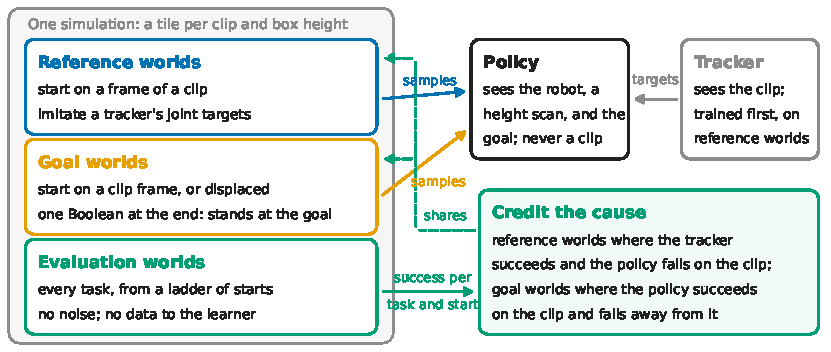
\includegraphics[width=0.92\textwidth]{figs/system.pdf}
\caption{Three kinds of worlds share one simulation and one policy. Reference worlds and goal worlds train it; evaluation worlds measure it on every task, and their success rates set how many worlds of each kind every task gets.}
\label{fig:system}
\end{figure*}
\section{Problem and Benchmark}
\label{sec:benchmark}

\textbf{Robot and simulation.} The robot is the 29-DoF Unitree G1 (34\,kg). The policy sets joint position targets at 30\,Hz for PD controllers; physics runs at 120\,Hz in MuJoCo Warp through Isaac Lab~\cite{isaaclab}. Climbing loads the thighs, forearms, and upper arms, so we use the asset's collision geometry for every link; with the reduced geometry that is common for locomotion, thighs and forearms pass through the box and our tracker does not climb.

\textbf{Clips and terrain.} The terrain clips of OmniRetarget~\cite{omniretarget} show a person, retargeted to the G1, climbing onto and over boxes, each clip at five scales of the box height (0.8 to 1.2). We place the boxes of every clip and scale on a tile of one terrain mesh, so a world is a robot on a tile (Fig.~\ref{fig:system}).

\textbf{Tasks.} In \clipsall{} of the 29 clips the robot stands upright on a box at some point. A \emph{task} is such a clip at one scale: start on the first frame, standing on the ground, and stand on the box where the clip does. This gives \tasksall{} tasks with boxes from 0.38 to 1.14\,m.

\textbf{Success.} An episode lasts as long as the clip takes to reach the goal frame plus two seconds. It \emph{succeeds} if, at its last step, the pelvis is within 0.3\,m of the goal pose in the ground plane and 0.15\,m in height, and is upright. Success therefore requires standing still on the box for the remaining time, not touching it.

\textbf{Evaluation.} We report success from two kinds of starts: the first frame of the clip (\emph{clip start}), and that frame moved by up to 0.5\,m along each ground axis and turned by up to 0.5\,rad (\emph{displaced start}). A tracker can be expected to solve the first and not the second.

\textbf{Observations and actions.} The policy observes the pelvis height and velocity, projected gravity, joint positions and velocities, the positions of the bodies relative to the pelvis, a $2.0\times1.2$\,m height scan around the pelvis, the goal pose relative to the pelvis, and its last action: 541 numbers. It does not observe a clip, a phase, or time. Actions are offsets of 0.5\,rad scale from a standing pose. These observations include quantities a robot must estimate; like most trackers, this is a state-based policy in simulation.

\section{Method}
\label{sec:method}

\subsection{One task definition, three kinds of worlds}

All worlds share one policy, one observation space, and one terrain. What a world does is set per episode by a few numbers that the learner writes for it: the tile, the frame to start on, the goal frame, the weights of its rewards, and when it ends. A world can therefore change kind at any reset, and the share of each kind is a number the learner may change at any time, per task. The step of all worlds, including the rewards and resets, is recorded once as a GPU graph and replayed.

\textbf{Reference worlds} start on a frame of the task's clip, drawn uniformly up to the goal frame. They receive the tracking reward of~\cite{deepmimic}-style trackers (joint positions and velocities, body positions, root velocity) and end when the bodies are 0.3\,m from the clip on average. In addition, a tracker gives the joint targets it would command in the current state, and the policy's loss adds the squared distance of its mean action to them (Sec.~\ref{sec:tracker}).

\textbf{Goal worlds} receive 20 at the last step of an episode that succeeds, 0.5 per second of survival, and a small penalty for tilt; they end when the pelvis is below 0.3\,m. Half start on a frame of the clip, as above; the other half start on the first frame, displaced as in the evaluation. The first half gives the Boolean a signal before the policy can do the whole task, the second trains what the evaluation asks for.

\textbf{Evaluation worlds} act without exploration noise and give no data to the learner. For every task they start from a ladder of rungs: the clip start, three frames a quarter, a half and three quarters of the way to the goal, and displaced starts. We write $L_\tau$ for the success of task $\tau$ averaged over the four on-clip rungs and $D_\tau$ for its success from displaced starts.

\subsection{A tracker teaches the reference worlds}
\label{sec:tracker}

A policy that cannot see the clip must recover from its own state which part of the motion comes next. It can learn this from the tracking reward: with reference worlds only, it climbs in two of three runs (Sec.~\ref{sec:cause}). But goal worlds added from the first iteration destroy that learning, as~\cite{wang2026generalizing} report: with an even split and the tracking reward, our policy learns nothing. Hybrid methods answer with a schedule that withholds the goal worlds. We give the reference worlds a stronger signal instead.

We first train a tracker with reference worlds only. It observes the tracked frame, and its action is a correction to the joint positions of that frame, the form of the successors of~\cite{deepmimic}; a policy without a clip cannot share this action space. We then use the tracker as a teacher. In a reference world the teacher is evaluated on the policy's state, as in DAgger~\cite{dagger}, and its joint targets, expressed in the policy's action space, are a regression target for the mean action. The policy still acts and still receives the tracking reward. The teacher costs one extra network evaluation per step and no simulation. With it, an even split works from the first iteration, and the share of reference worlds becomes a question of how fast, which the next section answers, rather than of whether.

\subsection{Credit the cause}
\label{sec:rule}

Which kind of world should a task get? Section~\ref{sec:cause} measures what each kind causes: reference worlds give success from the frames of the clip and little away from it; goal worlds give success away from the clip, but only once the policy can do the motion; goal worlds without it give nothing. The rule states this as an allocation. Let $T_\tau$ be the success of the teacher on task $\tau$. Reference worlds are wanted where the teacher can show the motion and the policy cannot yet do it, and goal worlds where the policy can do the motion but not away from the clip:
\begin{align}
w^{\text{ref}}_\tau &= T_\tau\,(1 - L_\tau), &
w^{\text{goal}}_\tau &= (L_\tau + \epsilon)\,(1 - D_\tau).
\end{align}
The share of reference worlds is $p = \sum_\tau w^{\text{ref}}_\tau / \sum_\tau (w^{\text{ref}}_\tau + w^{\text{goal}}_\tau)$, never below 0.05, and the worlds of a kind are spread over the tasks in proportion to $w$ plus a small floor. $L$ and $D$ are the success rates of the evaluation worlds since the last update, smoothed over updates; we update every 100 iterations. The rule has no schedule and no target: it starts with references, because nothing else can be taught, and moves to goals as the evaluation shows the motion arriving. Without the two gates ($T_\tau$ and $L_\tau+\epsilon$) it reduces to splitting the worlds by the two failure rates, which we also report. We use $\epsilon = 0.1$, and $T_\tau = 1$ in the development experiments, where the teacher solves every task.

\textbf{Measuring instead of modelling.} The rule encodes causes that we measured once. The direct alternative measures them continuously: two learners, each with half of the worlds, train with shares $p+\delta$ and $p-\delta$; every 100 iterations the one whose evaluation worlds succeed more often gives the other its policy, and $p$ moves towards its share. This is an intervention with a control, and we use it to check the direction the rule takes. It costs twice the samples: at our batch size, a learner with half the worlds needs as many samples as one with all of them.

\subsection{Learner}

We use PPO~\cite{ppo} with GAE~\cite{gae}, rollouts of 6 steps of 4{,}096 training worlds, four epochs of four minibatches, an adaptive learning rate, and an asymmetric critic~\cite{pinto2018asymmetric} that also sees the kind of episode, its remaining time, and the tracked frame. The discount is 0.95 in reference worlds and 0.995 in goal worlds. Short rollouts with a high learning-rate ceiling learned markedly faster per sample in our first tests than the settings common for locomotion~\cite{rudin2022minutes}. Advantages are normalised over all worlds, so a kind of world whose rewards have not started yet stays quiet.

\section{Experiments}
\label{sec:experiments}

\textbf{Setup.} Development experiments use one clip, a climb onto a 0.84\,m box, at its five box heights (0.67 to 1.01\,m): five tasks. They train 4{,}096 worlds for 59 million samples with 320 evaluation worlds on the side, three seeds per setting. Samples count the steps of training worlds; evaluation worlds add 8\% of simulation that we do not count. The tracker that teaches the reference worlds is trained once, for 74 million samples, and shared by all settings. ``Success holds from $n$ samples'' means that the evaluation success, logged every 2.5 million samples, stays at or above the level from $n$ on. All-clip experiments use 8{,}192 training worlds and 1{,}680 evaluation worlds. Everything runs on one RTX PRO 6000 GPU.

\subsection{What each kind of world causes}
\label{sec:cause}

Table~\ref{tab:cause} isolates the kinds of worlds on the development tasks.

\emph{Goal worlds alone learn nothing.} With the Boolean, the survival term, and starts on clip frames up to the one before the goal, success is \causeGoal{} from every rung in every seed, including starts where the robot already stands on the box. A humanoid does not stay upright by chance for the second that separates it from the first reward.

\emph{A tracker solves the clip start and nothing else.} It succeeds in \causeTrackerClip{} of episodes from the first frame and \causeTrackerAway{} from displaced starts; it follows the clip where the clip is, not where the robot is.

\emph{Reference worlds give the motion to a policy that cannot see the clip.} Trained on reference worlds only, the policy reaches \causeRefClip{} from the clip start. It has learned which motion belongs to which state. From displaced starts it reaches \causeRefAway{}: more than the tracker, because its goal is relative to the robot, and far from solved.

\emph{Goal worlds turn the motion into the task.} With goal worlds for half of the worlds, success from displaced starts rises to \causeHybridAway{} while the clip start stays at \causeHybridClip{}.

\emph{The teacher is what lets the two kinds mix from the start.} \causeNoTeacher{}

So the causes are separable and ordered: reference worlds cause success on the clip, goal worlds cause success away from it, and the second needs the first. This is the structure the rule of Sec.~\ref{sec:rule} assumes.

\begin{table}[t]
\centering
\caption{What each kind of world causes: success on the development tasks after 59 million samples. Mean of three seeds, with their range; the tracker is one run.}
\label{tab:cause}
\begin{tabular}{@{}lcc@{}}
\toprule
Worlds that train the policy & Clip start & Displaced start \\
\midrule
Goal worlds only & 0.00 \,{\scriptsize(0.00--0.00)} & 0.00 \,{\scriptsize(0.00--0.00)} \\
Tracker (observes the clip) & 0.84 & 0.05 \\
\midrule
Reference worlds, tracking reward & 0.59 \,{\scriptsize(0.00--0.93)} & 0.29 \,{\scriptsize(0.00--0.45)} \\
Reference worlds, teacher & 0.92 \,{\scriptsize(0.91--0.93)} & 0.25 \,{\scriptsize(0.24--0.26)} \\
Both, tracking reward & 0.00 \,{\scriptsize(0.00--0.00)} & 0.00 \,{\scriptsize(0.00--0.00)} \\
Both, teacher & 0.98 \,{\scriptsize(0.96--0.99)} & 0.92 \,{\scriptsize(0.92--0.93)} \\
\bottomrule
\end{tabular}

\end{table}

\subsection{The share is a strong and one-sided lever}
\label{sec:share}

Fig.~\ref{fig:sweep} sweeps a fixed share of reference worlds. With a share of 0.10 the policy learns nothing in the budget: the goal worlds, which cannot yet be rewarded, outnumber the worlds that teach. With 0.25 and 0.50 it reaches both success levels. With 0.75 it is slow away from the clip, and with 1.00 it stays tied to the clip. A hand-set share therefore has a cliff on one side and a slope on the other, and a practitioner finds the safe region by a sweep of full training runs.

\begin{figure}[t]
\centering
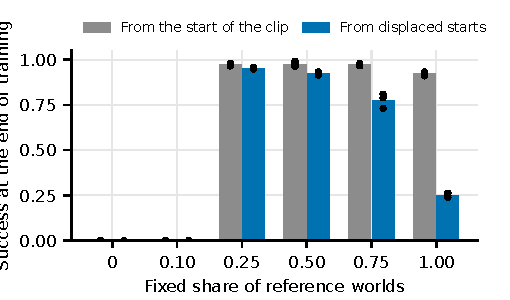
\includegraphics[width=\columnwidth]{figs/sweep_dev.pdf}
\caption{Success at the end of training for fixed shares of reference worlds. Bars are means of three seeds, dots the seeds.}
\label{fig:sweep}
\end{figure}

\subsection{Allocation by the evaluation against hand schedules}
\label{sec:schedules}

Table~\ref{tab:schedules} and Fig.~\ref{fig:schedules} compare ways to set the share. All use the same reference worlds, teacher, and goal worlds.

\emph{Hand schedules.} ``Two stages'' trains reference worlds alone for two thirds of the budget and then an even split, the proportions of~\cite{hil}. ``Tracking progress'' lowers the share from 1.0 to 0.5 in steps while fewer than 30\% of the reference episodes lose their clip, in the manner of~\cite{wang2026generalizing}. Both reach the clip-start level early, because they start with references only, and the displaced level late, because they hold goal worlds back by a clock or by a statistic of the wrong task.

\emph{The credit rule} reads the evaluation worlds every 100 iterations. \scheduleSentence{}

\emph{Trial learners.} The two learners that try shares 0.15 above and below the current one choose the reference-heavy share for the first \trialSamples{} million samples and then walk the share down to about 0.2 (Fig.~\ref{fig:schedules}, right). This is the direction the rule takes, measured by intervention rather than assumed. Its cost is as predicted: each learner has half of the worlds, and the pair needs \trialCost{} the samples of the rule.

\emph{Without the teacher} the picture changes (lower block of Table~\ref{tab:schedules}). \noTeacherSentence{}

\begin{table}[t]
\centering
\caption{Ways to set the share of reference worlds on the development tasks. Mean and range of the seeds: three with the teacher, two or three without. [$n/m$]: the $n$ of $m$ seeds that got there; ``never'': none within 59 million samples.}
\label{tab:schedules}
\setlength{\tabcolsep}{3pt}
\resizebox{\columnwidth}{!}{\begin{tabular}{@{}lcccc@{}}
\toprule
 & \multicolumn{2}{c}{Samples (M) until success holds} & \multicolumn{2}{c}{Success at 59\,M} \\
Share of reference worlds & clip $\geq$0.9 & displaced $\geq$0.8 & clip & displaced \\
\midrule
Goal worlds only & never & never & 0.00 \,{\scriptsize(0.00--0.00)} & 0.00 \,{\scriptsize(0.00--0.00)} \\
\midrule
\multicolumn{5}{@{}l}{\emph{Reference worlds taught by a tracker}} \\
Fixed share 0.10 & never & never & 0.00 \,{\scriptsize(0.00--0.00)} & 0.00 \,{\scriptsize(0.00--0.00)} \\
Fixed share 0.25 & 35 \,{\scriptsize(32--39)} & 38 \,{\scriptsize(34--42)} & 0.98 \,{\scriptsize(0.97--0.98)} & 0.95 \,{\scriptsize(0.95--0.96)} \\
Fixed share 0.50 & 26 \,{\scriptsize(25--27)} & 37 \,{\scriptsize(37--37)} & 0.98 \,{\scriptsize(0.96--0.99)} & 0.92 \,{\scriptsize(0.92--0.93)} \\
Fixed share 0.75 & 34 \,{\scriptsize(29--39)} & 57 \,{\scriptsize[1/3]} & 0.97 \,{\scriptsize(0.97--0.98)} & 0.78 \,{\scriptsize(0.73--0.81)} \\
Fixed share 1.00 & 50 \,{\scriptsize(47--57)} & never & 0.92 \,{\scriptsize(0.91--0.93)} & 0.25 \,{\scriptsize(0.24--0.26)} \\
Two stages~\cite{hil} & 44 \,{\scriptsize(42--47)} & 53 \,{\scriptsize(52--57)} & 0.98 \,{\scriptsize(0.97--0.98)} & 0.85 \,{\scriptsize(0.84--0.87)} \\
Tracking progress~\cite{wang2026generalizing} & 31 \,{\scriptsize(29--32)} & 43 \,{\scriptsize(42--47)} & 0.98 \,{\scriptsize(0.97--0.99)} & 0.91 \,{\scriptsize(0.90--0.91)} \\
Two trial learners & 51 \,{\scriptsize(47--54)} & 45 \,{\scriptsize(42--49)} & 0.95 \,{\scriptsize(0.95--0.96)} & 0.88 \,{\scriptsize(0.86--0.89)} \\
Credit rule without gates & 25 \,{\scriptsize(22--27)} & 27 \,{\scriptsize(27--27)} & 0.98 \,{\scriptsize(0.97--0.99)} & 0.95 \,{\scriptsize(0.94--0.96)} \\
Credit rule (ours) & 22 \,{\scriptsize(17--27)} & 22 \,{\scriptsize(22--22)} & 0.98 \,{\scriptsize(0.96--0.99)} & 0.95 \,{\scriptsize(0.94--0.97)} \\
\midrule
\multicolumn{5}{@{}l}{\emph{Reference worlds with the tracking reward only}} \\
Fixed share 0.50 & never & never & 0.00 \,{\scriptsize(0.00--0.00)} & 0.00 \,{\scriptsize(0.00--0.00)} \\
Fixed share 1.00 & 54 \,{\scriptsize(52--57)} \,{\scriptsize[2/3]} & never & 0.59 \,{\scriptsize(0.00--0.93)} & 0.29 \,{\scriptsize(0.00--0.45)} \\
Two stages~\cite{hil} & 47 \,{\scriptsize[1/2]} & 57 \,{\scriptsize[1/2]} & 0.49 \,{\scriptsize(0.00--0.98)} & 0.41 \,{\scriptsize(0.00--0.82)} \\
Tracking progress~\cite{wang2026generalizing} & never & never & 0.46 \,{\scriptsize(0.00--0.91)} & 0.24 \,{\scriptsize(0.00--0.47)} \\
Credit rule without gates & never & never & 0.00 \,{\scriptsize(0.00--0.00)} & 0.00 \,{\scriptsize(0.00--0.00)} \\
Credit rule & never & never & 0.00 \,{\scriptsize(0.00--0.00)} & 0.00 \,{\scriptsize(0.00--0.00)} \\
\bottomrule
\end{tabular}
}
\end{table}

\begin{figure*}[t]
\centering
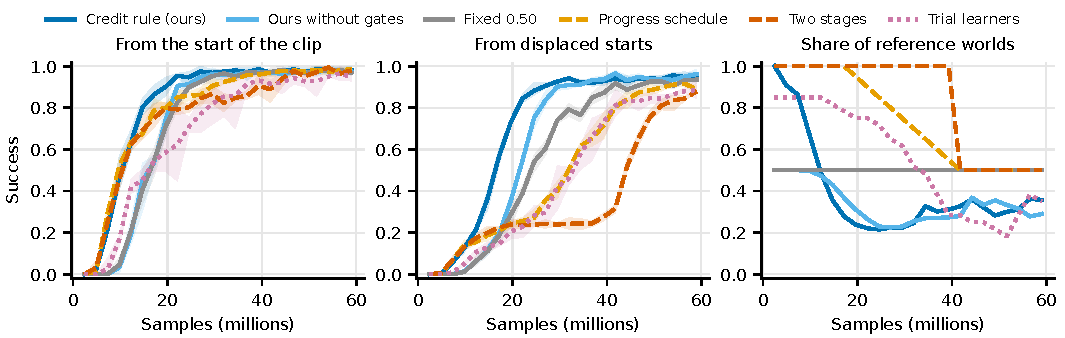
\includegraphics[width=\textwidth]{figs/schedules_dev.pdf}
\caption{Success from the clip start and from displaced starts during training, and the share of reference worlds that each method uses. Lines are means of three seeds, bands their range.}
\label{fig:schedules}
\end{figure*}

\subsection{Away from the clip}

Fig.~\ref{fig:displaced} moves the start further than training did. The policy was trained with displacements up to 0.5\,m and 0.5\,rad. It succeeds in \displacedHalf{} of episodes at that range, \displacedThreeQuarters{} at 0.75, and \displacedOne{} at 1.0; the tracker is at \displacedTrackerQuarter{} already at 0.25 and at \displacedTrackerOne{} at 1.0. Fig.~\ref{fig:teaser} shows one such episode.

\begin{figure}[t]
\centering
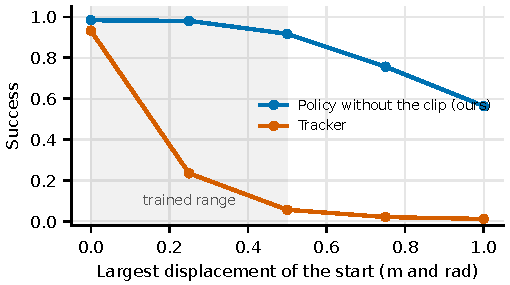
\includegraphics[width=\columnwidth]{figs/displaced.pdf}
\caption{Success from starts displaced by up to the amount on the horizontal axis, along both ground axes and in heading, over about a thousand episodes per point.}
\label{fig:displaced}
\end{figure}

\subsection{All clips, one policy}
\label{sec:all}

We train one tracker and then one policy on all \tasksall{} tasks, with 8{,}192 training worlds. The credit rule now also spreads the worlds of each kind over the tasks.

\emph{The tracker.} After \fullTrackerSamples{} million samples the tracker succeeds from the clip start in \fullTrackerClip{} of episodes averaged over the tasks, and in \fullTrackerAway{} from displaced starts. It solves \fullTrackerSolved{} of the \tasksall{} tasks at 0.5 or better. The tasks it does not solve are mostly the tallest boxes and three clips whose climbs it never completes; a second stage of training on the partly solved tasks gained 0.01 per 25 million samples and was stopped.

\emph{The policy.} Fig.~\ref{fig:full} shows the policy trained with the credit rule and this tracker as its teacher. \fullSentence{}

\emph{Past the teacher.} Fig.~\ref{fig:fulltasks} shows where. \fullTasksSentence{} The rule's gate gives these tasks few reference worlds, because the teacher cannot show them; what solves them is the Boolean in goal worlds, on a policy that has learned to climb elsewhere. A tracker cannot do this: it has no goal to be rewarded for.

\begin{figure}[t]
\centering
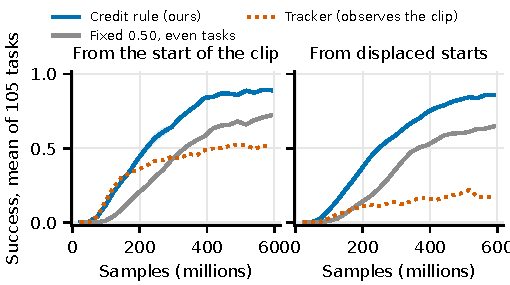
\includegraphics[width=\columnwidth]{figs/full_curves.pdf}
\caption{All \tasksall{} tasks, one policy. The policy does not observe a clip; the tracker that teaches it does. Credit rule: mean and range of \seedsAll{} seeds.}
\label{fig:full}
\end{figure}

\begin{figure*}[t]
\centering
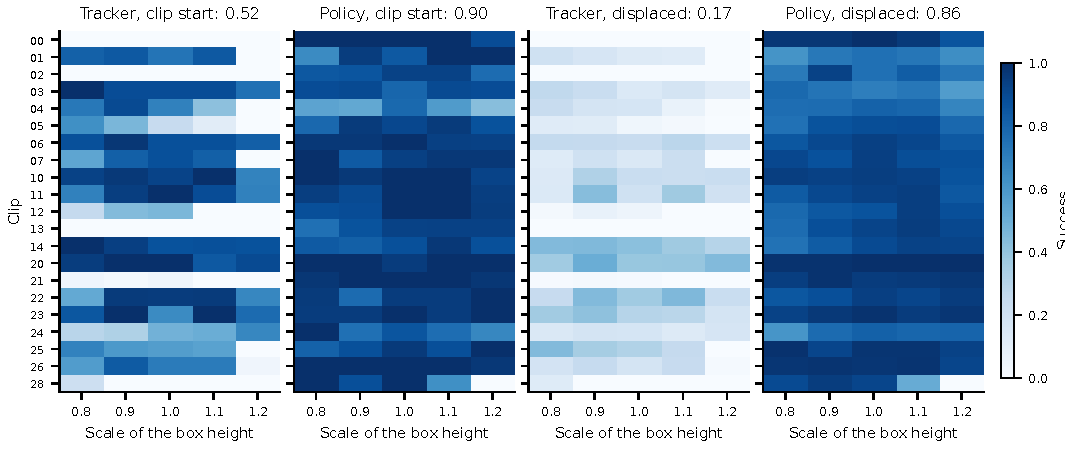
\includegraphics[width=\textwidth]{figs/full_tasks.pdf}
\caption{Success on every task at the end of training: a row per clip, a column per scale of the box height, and the mean over the tasks in each title. The policy is its first seed.}
\label{fig:fulltasks}
\end{figure*}

\subsection{Tasks that no world trained}

Does the policy climb boxes it never trained on? We repeat the run with tasks held out: no reference world and no goal world is ever placed on them, and the evaluation worlds still measure them (Table~\ref{tab:heldout}). \heldoutSentence{}

\begin{table}[t]
\centering
\caption{Tasks held out of training: no world of either kind is placed on them. Success averaged over the tasks.}
\label{tab:heldout}
\setlength{\tabcolsep}{4pt}
\input{figs/table_heldout}
\end{table}

\subsection{Training time}

\timeSentence{}


\section{What Did Not Work}

We list what failed, because several of these are natural first choices. (i) A per-step penalty for tilt with termination on a fall rewards falling early, since every step survived costs reward; we replaced it with a survival term, and goal worlds alone still learned nothing. (ii) Starting worlds on the stretch of the clip where the evaluation ladder shows episodes being lost, a reverse curriculum read from the ladder, was worse than uniform starts for the tracker: it learned the last stretch first and never the ones before (0.00 against \lossStarts{} from the clip start at 25 million samples). (iii) With the reduced collision geometry of the robot, the tracker lost the clip in half of its episodes, at the climb, against one in twenty with the full geometry.

\section{Limitations}
\label{sec:limits}

All results are in simulation, with a state-based policy that observes quantities a robot must estimate, without domain randomisation; we have not run the policy on hardware. The rule needs the teacher: with the tracking reward alone it learns nothing, because it places a few goal worlds from the first iteration. The rule encodes two causal relations that we measured on these tasks; a task family in which goal worlds teach without references, or references mislead, needs them measured again, which the trial learners do at twice the cost. Success is defined by the pose of the pelvis, so the policy is not asked to move like the clip, and we did not measure how closely it does. The displaced starts are within a metre of the clip start and always in front of the box. We report three seeds for the development experiments, \seedsAll{} for the policy on all clips, and one for each other experiment on all clips. Without the teacher, the tracking reward taught the climb in some runs and not in others, and we do not know what separates them.

\section{Conclusion}

Clips can give a goal-driven policy what a Boolean reward cannot, but only through worlds that are there for a reason. We measured the reasons: reference worlds cause the motion, goal worlds cause its use away from the clip, and the second waits for the first. Stated as a rule that reads evaluation worlds, they replace the hand schedules of hybrid imitation, reach the same success in about half the samples with no setting to tune, and carry one policy past its teacher, onto tasks the teacher never solved. What the rule cannot do is start without a teacher. Removing that dependence and running the policy on the robot are the next steps.



\bibliographystyle{plainnat}
\bibliography{refs}

\end{document}
